\section{Introduction}
\label{bso_sec:intro}
% ====================

\begin{figure}[!htp]
\begin{center}
\begin{ccTexOnly}
  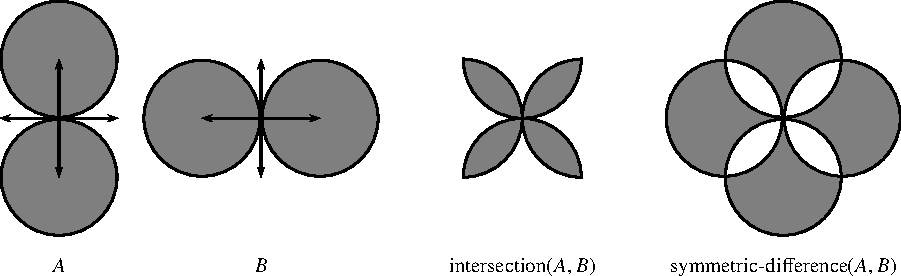
\includegraphics{Boolean_set_operations_2/fig/teaser}
\end{ccTexOnly}
\label{fig:teaser}
\begin{ccHtmlOnly}
  <p><center>
    <img src="./fig/teaser.gif" border=0 alt="Boolean Set-Operations">
  </center>
\end{ccHtmlOnly}
\caption{Examples of Boolean set-operations on general polygons.} 
\end{center}
\end{figure}

This package consists of the implementation of Boolean set-operations
on point sets bounded by $x$-monotone curves\footnote{A continuous
planar curve $C$ is {\em $x$-monotone} if every vertical line intersects it at
most once. We also allow vertical line segments, which are considered
{\em weakly} $x$-monotone.} in 2-dimensional Euclidean space. In particular,
it contains the implementation of {\em regularized} Boolean set-operations,
intersection predicates, and point containment predicates.
Figure~\ref{fig:teaser} shows simple examples of such operations.

A regularized Boolean set-operation $\mbox{op}^*$ can be obtained by
first taking the interior of the resultant point set of an {\em ordinary}
Boolean set-operation $(P\ \mbox{op}\ Q)$ and then by taking the
closure~\cite{cgal:h-sm-04}. That is,
$P\ \mbox{op}^*\ Q = \mbox{closure}(\mbox{interior} (P\ \mbox{op}\ Q))$.
Regularized Boolean set-operations appear in Constructive Solid
Geometry (CSG), because regular sets are closed under regularized
Boolean set-operations, and because regularization eliminates lower
dimensional features, namely isolated vertices and antennas, thus
simplifying and restricting the representation to physically meaningful
solids. Our package provides regularized operations on polygons and
general polygons, where the edges of a general polygon may be
general $x$-monotone curves, rather than being simple line segments.
Ordinary Boolean set-operations, which distinguish between the
interior and the boundary of a polygon, are not implemented within this
package. The \ccc{Nef_2} package supports these operations for (linear)
polygons; see Chapter~\ref{chap:nef_2}.

In the rest of this chapter we use --- unless otherwise stated --- the
traditional notation to designate regularized operations; e.g., $P \cap Q$
means the {\em regularized} intersection of $P$ and $Q$.

A polygon $P$ is said to be {\em simple} (or Jordan) if the only
points of the plane belonging to two polygon edges of $P$ are the
polygon vertices of $P$. Namely, the polygon edges are pairwise
disjoint in their interior. Such a polygon has a well-defined interior
and exterior and is topologically equivalent to a disk. A polygon in our
context must be simple and its vertices must be ordered in a
counterclockwise direction around the interior of the polygon.
 
\lcTex{%
  \setlength{\BooleanSetOpsWidthRight}{1.4cm}
  \setlength{\BooleanSetOpsWidthLeft}{\BooleanSetOpsWidthLineReal}
  \addtolength{\BooleanSetOpsWidthLeft}{-\BooleanSetOpsWidthRight}
  \begin{minipage}{\BooleanSetOpsWidthLeft}
}
\label{fig:non_strictly_simple_polygon}
\begin{ccHtmlOnly}
  <p><center>
    <img src="./fig/non_strictly_simple.gif" border=0 alt="A non strictly simple polygon" align=right>
  </center>
\end{ccHtmlOnly}
The counterclockwise cyclic sequence of alternating polygon edges and
polygon vertices is referred to as the polygon {\em boundary}.
A polygon whose boundary contains the same vertex twice or more is connected
and simple but not necessarily strictly simple, such as the polygon depicted
on the right.  We extend the notion of a polygon to a point set in $\real^2$
that has  a topology of a polygon and its boundary edges must map to
$x$-monotone curves, and refer to it as a {\em general polygon}. We
sometimes use the term {\em polygon} instead of general polygon for
simplicity hereafter.
\lcTex{%
  \end{minipage}\hspace{\BooleanSetOpsMinipageSpace}
  \begin{minipage}{\BooleanSetOpsWidthRight}
    \begin{center}
    
\includegraphics{Boolean_set_operations_2/fig/non_strictly_simple}
    \end{center}
%    A non strictly simple polygon.
  \end{minipage}
}

Our package supports the following Boolean set-operations on two point
sets $P$ and $Q$ that are comprised of general polygons:
\begin{description}
\item[Intersection] computes the intersection $R = P \cap Q$.
\item[Join] computes the union $R = P \cup Q$.
\item [Difference] computes the difference $R = P \setminus Q$.
\item [Symmetric Difference] computes the symmetric
  \ccHtmlNoLinksFrom{difference} $P = P \oplus Q = (P \setminus Q) \cup (Q \setminus P)$.
\item[Complement] computes the complement
  \lcTex{$R = \overline{P}$.}
  \lcRawHtml{<i>R = <span style="text-decoration: overline;">P</span>.</i>}
\item [Intersection predicate] tests whether the two sets $P$ and $Q$
  overlap, distinguishing three possible scenarios: (i) the two sets
  intersect on their interior (that is, their regularized intersection
  is not empty $P \cap Q \neq \emptyset$); (ii) the boundaries of two
  sets intersect but their interiors are disjoint; namely they have a
  finite number of common points or even share a boundary curve (still
  in this case $P \cap Q = \emptyset$; and (iii) the two sets are
  disjoint.
\end{description}
In general, the set $R$, resulting from a regularized Boolean
set-operation, is considered as being a closed point-set.

In the rest of this chapter we review the Boolean set-operations package
in more depth. In Section~\ref{bso_sec:bso_lin} we focus on Boolean 
set-operations on linear polygons, introducing the notion of polygons with 
holes and of a general polygon set. Section~\ref{bso_sec:bso_gen}
introduces general polygons.
We first discuss polygons whose edges are either line segements or circular
arcs and then explain how to construct and use general polygons whose edges
can be arbitrary $x$-monotone curves.
